\subsection{Results on \benchmarkname}
\vspace{-0.15cm}
\label{sec:experiments_drawbench}

\begin{figure}[tb]
    \centering
    \begin{tabularx}{\linewidth}{XXXX}
        \centering
        \begin{subfigure}[t]{0.25\textwidth}
        \centering
        \hspace*{-9pt}\input{figures/pgfplots/drawit_vs_dalle2_twoway.tex}    
        \label{fig:drawit_vs_dalle2_drawbench}
        \end{subfigure} & 
        \begin{subfigure}[t]{0.25\textwidth}
        \centering
        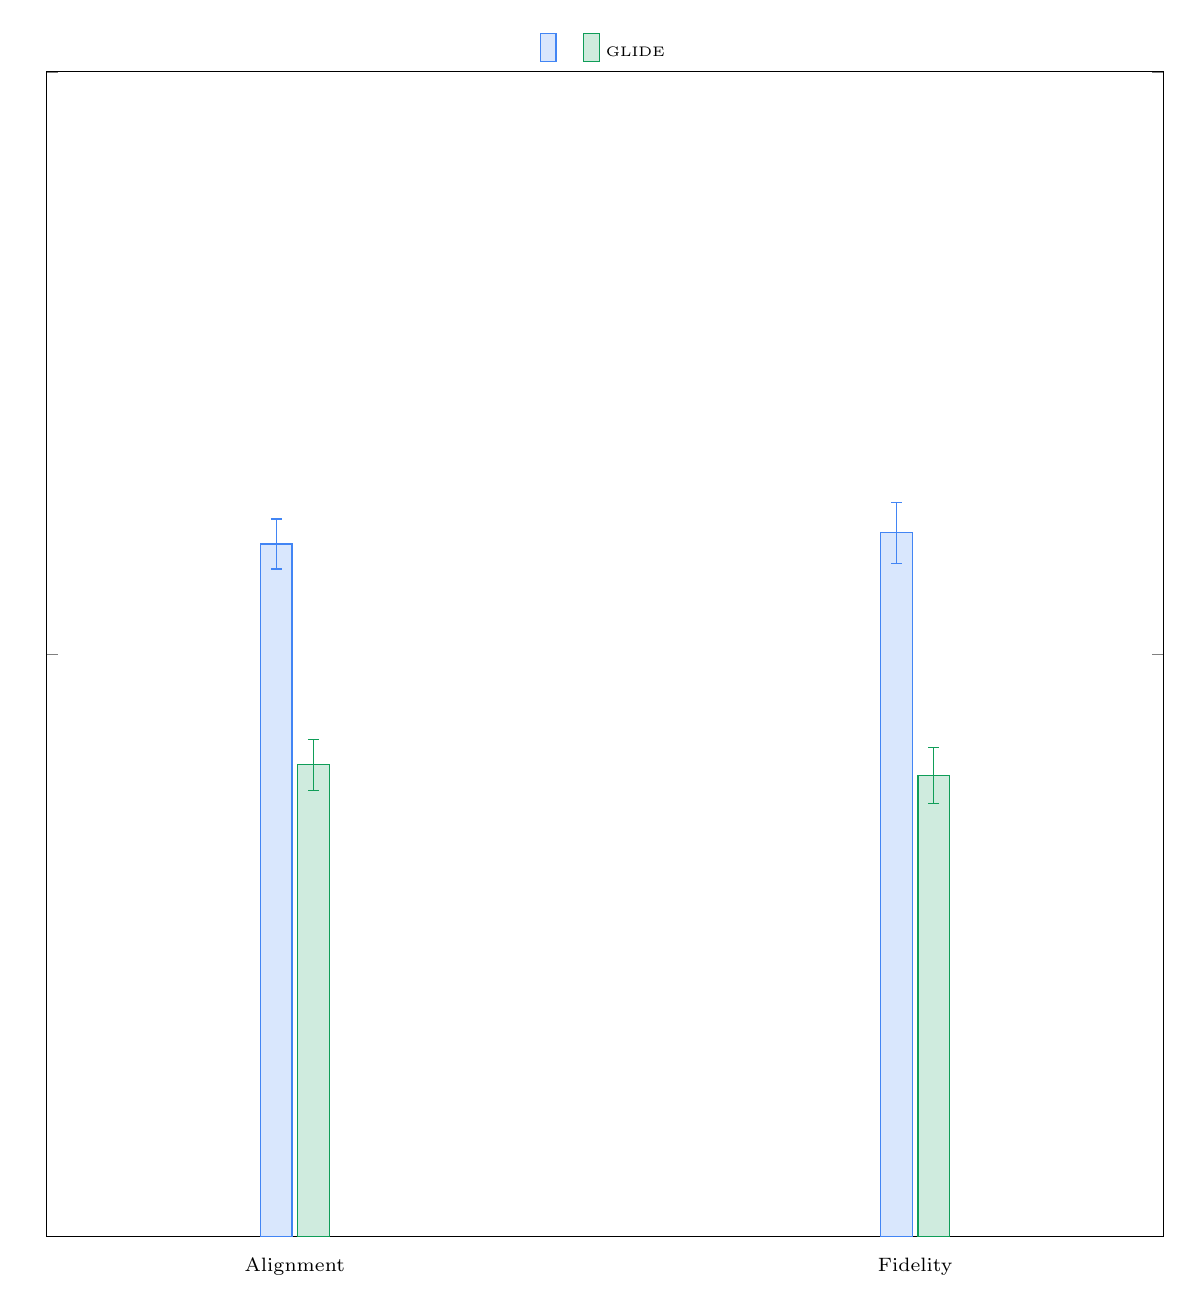
\begin{tikzpicture}

\definecolor{google_blue}{RGB}{66,133,244}
\definecolor{google_red}{RGB}{219,68,55}
\definecolor{google_yellow}{RGB}{194,144,0}
\definecolor{google_green}{RGB}{15,157,88}

\begin{axis}[
name=fidelity,
width=1.3\textwidth,
height=1.35\textwidth,
ybar,
ymin=0.0,
ymax=1.0,
xtick={1, 2},
xtick style={draw=none},
xticklabels={Alignment, Fidelity},
every tick label/.append style={font=\scriptsize},
ytick={0,0.5,1},
yticklabels={},
legend style={font=\tiny},
legend cell align=left,
legend image code/.code={
    \draw [#1] (0cm, -0.1cm) rectangle (0.2cm, 0.25cm);
},
legend style={
draw=none,
at={(0.5, 1.0)},anchor=south,
legend columns=3,
/tikz/every even column/.append style={column sep=0.2cm}
},
bar width=0.4cm,
enlarge x limits={abs=0.4},
]
\addplot+[
    fill=google_blue,
    fill opacity=0.2,
    draw=google_blue,
    error bars/error bar style={google_blue},
    error bars/.cd,
    y dir=both,
    y explicit
] coordinates {
(1.0,0.5945) +- (1.0, 0.02145839465123118)
(2.0,0.604) +- (2.0, 0.02598245656099196)
};

\addplot+[
fill=google_green,fill opacity=0.2,draw=google_green,
    error bars/error bar style={google_green},
    error bars/.cd,
    y dir=both,
    y explicit
] coordinates {
(1.0,0.405) +- (1.0, 0.021982563782935984)
(2.0,0.396) +- (2.0, 0.02406971888310527)
};


\legend{\name, GLIDE}
\end{axis}

\end{tikzpicture}


    
        \label{fig:drawit_vs_glide_drawbench}
        \end{subfigure} & 
        \begin{subfigure}[t]{0.25\textwidth}
        \centering
        \input{figures/pgfplots/drawit_vs_vqganclip_twoway}
        \label{fig:drawit_vs_vaganclip_drawbench}
        \end{subfigure} &
        \begin{subfigure}[t]{0.25\textwidth}
        \centering
        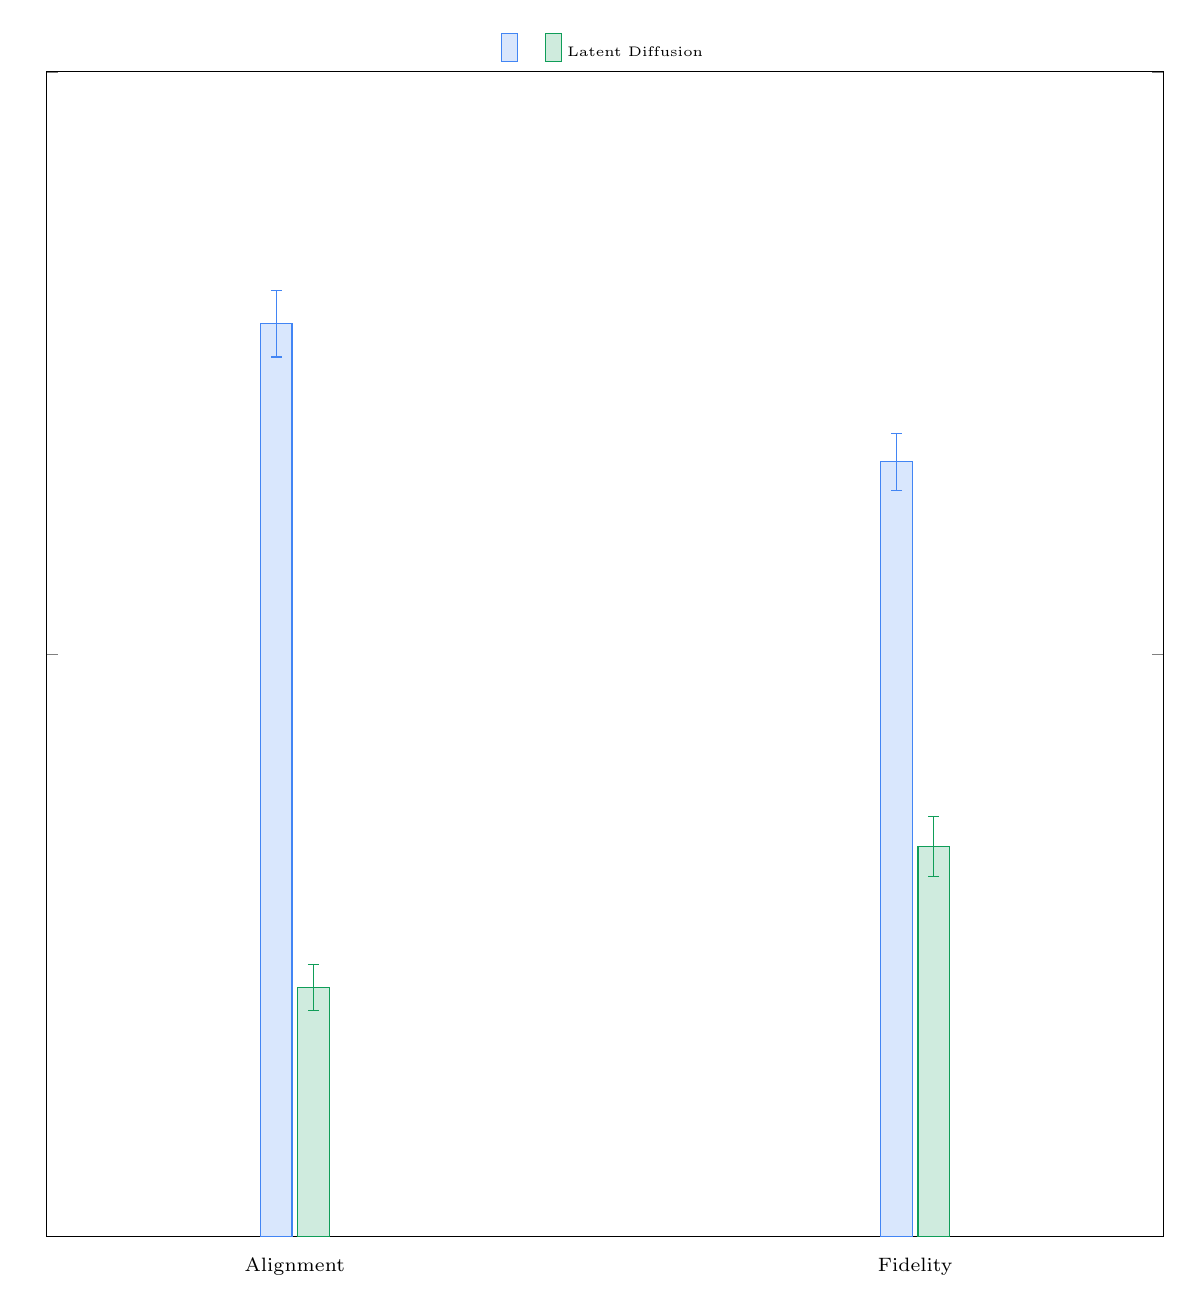
\begin{tikzpicture}

\definecolor{google_blue}{RGB}{66,133,244}
\definecolor{google_red}{RGB}{219,68,55}
\definecolor{google_yellow}{RGB}{194,144,0}
\definecolor{google_green}{RGB}{15,157,88}

\begin{axis}[
name=fidelity,
width=1.3\textwidth,
height=1.35\textwidth,
ybar,
ymin=0.0,
ymax=1.0,
xtick={1, 2},
xtick style={draw=none},
xticklabels={Alignment, Fidelity},
every tick label/.append style={font=\scriptsize},
ytick={0,0.5,1},
yticklabels={},
legend style={font=\tiny},
legend cell align=left,
legend image code/.code={
    \draw [#1] (0cm, -0.1cm) rectangle (0.2cm, 0.25cm);
},
legend style={
draw=none,
at={(0.5, 1.0)},anchor=south,
legend columns=3,
/tikz/every even column/.append style={column sep=0.2cm}
},
bar width=0.4cm,
enlarge x limits={abs=0.4},
]

\addplot+[
    fill=google_blue,
    fill opacity=0.2,
    draw=google_blue,
    error bars/error bar style={google_blue},
    error bars/.cd,
    y dir=both,
    y explicit
] coordinates {
(1.0,0.7837) +- (1.0, 0.028497994689556643)
(2.0,0.6652) +- (2.0, 0.02454522731413525)
};

\addplot+[
fill=google_green,fill opacity=0.2,draw=google_green,
    error bars/error bar style={google_green},
    error bars/.cd,
    y dir=both,
    y explicit
] coordinates {
(1.0,0.2136) +- (1.0, 0.01993785825157147)
(2.0,0.3348) +- (2.0, 0.025427213103106437)
};

\legend{\name, Latent Diffusion}
\end{axis}

\end{tikzpicture}
        \label{fig:drawit_vs_latentdiffusion_drawbench}
        \end{subfigure} \\
    \end{tabularx}
    \caption{Comparison between \name and DALL-E 2~\citep{ramesh-dalle2}, GLIDE~\citep{nichol-glide}, VQ-GAN+CLIP~\citep{crowson2022vqgan} and Latent Diffusion~\citep{rombach-cvpr-2022} on \benchmarkname: User preference rates (with 95\% confidence intervals) for image-text alignment and image fidelity.}
    \label{fig:drawbench-comparison}
    \vspace{-1em}
\end{figure}


Using \benchmarkname, we compare \name with \mbox{DALL-E 2} (the public version)~\cite{ramesh-dalle2}, \mbox{GLIDE}~\cite{nichol-glide}, \href{https://github.com/CompVis/latent-diffusion}{\color{black}{Latent Diffusion}}~\cite{rombach-cvpr-2022}, and \href{https://github.com/EleutherAI/vqgan-clip}{\color{black}{CLIP-guided VQ-GAN}}~\cite{crowson2022vqgan}. %
\cref{fig:drawbench-comparison} shows the human evaluation results for pairwise comparison of \name with each of the three models. We report the percentage of time raters prefer Model A, Model B, or are indifferent for both image fidelity and image-text alignment. We aggregate the scores across all the categories and raters. We find the human raters to exceedingly prefer \name over all others models in both image-text alignment and image fidelity. We refer the reader to \cref{sec:benchmark_comparison} for a more detailed category wise comparison and qualitative comparison. 
